\documentclass[11pt,a4paper]{article}

% CS6868 Research Mini-Project Report
\usepackage[utf8]{inputenc}
\usepackage[T1]{fontenc}
\usepackage[margin=1in]{geometry}
\usepackage{microtype}
\usepackage{lmodern}
\usepackage{amsmath,amssymb}
\usepackage{graphicx}
\usepackage{booktabs}
\usepackage{longtable}
\usepackage{array}
\usepackage{enumitem}
\usepackage{xcolor}
\usepackage{listings}
\usepackage{hyperref}
\usepackage[capitalise,noabbrev]{cleveref}

\graphicspath{{report_figures/}}

\hypersetup{
  colorlinks=true,
  linkcolor=black,
  citecolor=blue!60!black,
  urlcolor=blue!60!black,
}

\definecolor{codegray}{gray}{0.95}
\lstset{
  basicstyle=\ttfamily\small,
  backgroundcolor=\color{codegray},
  frame=single,
  framesep=4pt,
  breaklines=true,
  columns=fullflexible,
  keepspaces=true,
  showstringspaces=false,
}

\title{%
  \textbf{CS6868 Research Mini-Project} \\[0.3em]
  \Large Alloc-free-gc: Allocation-conscious Semi-space Garbage Collection in OxCaml%
}
\author{%
  Aditya Sawant \\ \texttt{CS23B003}
}
\date{\today}

\begin{document}
\maketitle

\begin{abstract}
\texttt{Alloc-free-gc} is an independent experimental garbage-collection
runtime for a small OCaml-style language implementation. The project studies
whether semi-space copying collection can be implemented in OCaml/OxCaml while
remaining competitive with a normal OCaml collector when heap ownership and the
allocation fast path are kept in C. The implementation compares five collector
variants: a normal OCaml collector, a zero-allocation OxCaml collector, an
off-heap metadata zero-allocation collector, a threaded off-heap collector, and
a stack-threaded collector service. On the checked-in benchmark matrix,
\texttt{zero\_offheap} has the best aggregate mean time, 4.914 seconds versus
5.127 seconds for \texttt{normal}. The improvement is modest, and the data have
one run per configuration, so the result is best read as directional rather
than statistically conclusive. The main conclusion is that allocation-conscious
OxCaml collection is viable, but zero-allocation annotations alone are not a
universal win; metadata placement and runtime coordination also matter.
\end{abstract}

% =============================================================================
\section{Goals}
\label{sec:goals}
% =============================================================================

The goal of this project was to build and evaluate a small garbage-collection
runtime in which the collector logic is written in OCaml/OxCaml rather than
entirely in C. The project focuses on a stop-the-world semi-space copying
collector, a design that is simple enough to implement completely while still
exercising important runtime-system concerns: root discovery, object copying,
pointer forwarding, heap-space swapping, and multi-threaded mutator
coordination.

The project connects to CS6868 topics in two ways. First, the runtime uses
threads, shared state, condition variables, and stop-the-world synchronization,
which are direct applications of concurrent programming and synchronization
ideas. Second, several variants change how the runtime crosses the boundary
between C and OCaml/OxCaml, which makes the project a practical study of
contention, coordination overhead, and implementation tradeoffs in systems with
multiple execution contexts.

The research question is:

\begin{quote}
Can a semi-space garbage collector implemented in allocation-conscious
OCaml/OxCaml be competitive with a normal OCaml implementation when all variants
share the same C allocation fast path?
\end{quote}

The secondary question is which optimization matters most: local zero-allocation
coding style, off-heap metadata, or persistent worker-thread execution.

% =============================================================================
\section{Background}
\label{sec:background}
% =============================================================================

\subsection{Semi-space Copying Collection}

The collector uses the classic semi-space copying strategy. The heap is divided
into two equal regions: from-space and to-space. Mutators allocate linearly in
from-space using a bump pointer. When allocation fails, mutators stop and the
collector copies all reachable objects into to-space. After collection,
from-space and to-space are swapped, and allocation resumes after the copied
live data.

The traversal is Cheney-style breadth-first copying~\cite{cheney1970}. The
collector maintains a \texttt{free\_ptr}, where the next copied object will be
placed, and a \texttt{scan\_ptr}, which walks through objects already copied to
to-space. Roots are copied first. Then the collector scans copied objects and
copies any reachable pointer fields that still point into the old from-space.

\begin{lstlisting}[language=C,caption={High-level semi-space collection sketch.},label={lst:cheney}]
free_ptr = to_space_start;
scan_ptr = to_space_start;

for root in roots:
  root = copy(root, &free_ptr);

while scan_ptr < free_ptr:
  obj = scan_ptr;
  for field in obj.pointer_fields:
    field = copy(field, &free_ptr);
  scan_ptr += object_size(obj);

swap(from_space, to_space);
current_heap_ptr = free_ptr - new_from_space;
\end{lstlisting}

\subsection{Runtime Representation}

The runtime uses an OCaml-style tagged-word representation. Integers have low
bit \(1\), while heap pointers have low bit \(0\). Heap pointers exposed to
program code point to the object body. The object header is stored one word
before the body and records the object size and tag.

During copying, the old object is converted into a forwarding object: the header
is overwritten with a forwarding marker, and the first payload slot stores the
new body pointer. Later visits to the same object can then return the forwarded
address without copying the object again.

\subsection{Root Tracking and Stop-the-world Collection}

Root tracking is explicit. Each mutator has a thread-local stack of root
addresses, a stack index, a return-value root slot, and an active/inactive flag.
The collector scans root addresses and updates them in place after moving
objects.

Collection is stop-the-world. When the allocation path cannot satisfy a request,
the requesting mutator marks a GC request and waits until all active mutators
reach a polling or allocation point. The selected collector variant then runs
with no concurrent mutation.

% =============================================================================
\section{Tasks Undertaken}
\label{sec:tasks}
% =============================================================================

\subsection{Implementation}

The project is organized into three layers.

\begin{itemize}[leftmargin=*]
  \item \textbf{Runtime layer}: \texttt{runtime.c} and \texttt{runtime.h}
  define tagged-value helpers, allocation entry points, mutator thread startup,
  explicit root registration, and stop-the-world coordination.
  \item \textbf{FFI and heap layer}: \texttt{gc\_ffi.c} embeds the OCaml/OxCaml
  runtime, owns the semi-space heap, exposes the \texttt{mmtk\_*} ABI consumed
  by the runtime layer, and provides no-allocation C stubs for raw memory
  access.
  \item \textbf{Collector layer}: one OCaml/OxCaml module is selected at build
  time through the Makefile variable \texttt{GC=}.
\end{itemize}

The implemented collector variants are:

\paragraph{Normal OCaml collector.}
\texttt{gc\_normal.ml} is the baseline. It implements the same semi-space
algorithm using ordinary OCaml references and arrays for metadata. This gives a
direct comparison point for the allocation-conscious variants.

\paragraph{Zero-allocation OxCaml collector.}
\texttt{gc.ml}, selected by \texttt{GC=zero}, rewrites the hot collection path
with OxCaml zero-allocation annotations. The copy function returns both the
updated pointer and next free pointer without allocating an OCaml pair.

\paragraph{Off-heap metadata collector.}
\texttt{gc\_zero\_offheap.ml}, selected by \texttt{GC=zero\_offheap}, moves
persistent metadata into malloc-backed memory. Static root slots, mutator root
stack pointers, stack-index pointers, return-root pointers, active-thread flags,
and counters are accessed through no-allocation C stubs.

\paragraph{Threaded off-heap collector.}
\texttt{GC=zero\_offheap\_threaded} uses the same off-heap collector but runs
collection through a persistent sleeping GC worker thread. Allocation failure
wakes the worker after mutators have stopped.

\paragraph{Stack-threaded collector service.}
\texttt{gc\_stack\_threaded.ml}, selected by
\texttt{GC=zero\_stack\_threaded}, runs collection inside a long-lived OxCaml
service loop. C owns mutator metadata; the OxCaml service thread performs only
collection when it receives a command.

\subsection{Testing and Verification}

Correctness was tested at three levels.

\begin{itemize}[leftmargin=*]
  \item \textbf{Smoke test}: \texttt{smoke\_test.c} allocates small linked
  objects, writes fields, and reads them back through the runtime API.
  \item \textbf{Single-threaded tree benchmark}: \texttt{benchmarks/binary\_tree.c}
  builds stretch, temporary, and long-lived trees and checks node-count
  traversals after allocation and collection.
  \item \textbf{Multi-threaded tree benchmark}:
  \texttt{benchmarks/binary\_tree\_multithreaded.c} runs the same allocation
  pattern across multiple worker threads and checks that all workers complete
  with the expected tree checksums.
\end{itemize}

The benchmark is not a formal proof of collector correctness, but it exercises
the important invariants for this project: roots must be updated after copying,
return values must survive allocation during nested calls, long-lived objects
must remain reachable, and stopped mutators must resume with valid pointers.

% =============================================================================
\section{Evaluation}
\label{sec:evaluation}
% =============================================================================

\subsection{Experimental Setup}

The main benchmark driver is
\texttt{benchmarking/run\_gc\_benchmark.sh}. It rebuilds
\texttt{binary\_tree\_multithreaded\_test} once per collector variant and records
elapsed wall-clock time. The checked-in result matrix uses:

\begin{itemize}[leftmargin=*]
  \item depths 11, 12, 13, and 14;
  \item mutator thread counts 1 through 8;
  \item variants \texttt{normal}, \texttt{zero}, \texttt{zero\_offheap},
  \texttt{zero\_offheap\_threaded}, and \texttt{zero\_stack\_threaded};
  \item one run per configuration.
\end{itemize}

The plotting script \texttt{benchmarking/plot\_gc\_benchmark.py} produces
per-depth time plots, summary statistics, and normal-relative speedup ratios.
Since the checked-in data have one run per configuration, the evaluation should
be read as directional. Repeated measurements are required for strong
quantitative claims.

\subsection{Pilot Benchmark}

An older pilot run compared only the normal OCaml and zero-allocation OxCaml
collectors. It is included because it was the first measurement of whether
zero-allocation annotations helped end-to-end runtime.

\begin{figure}[h]
  \centering
  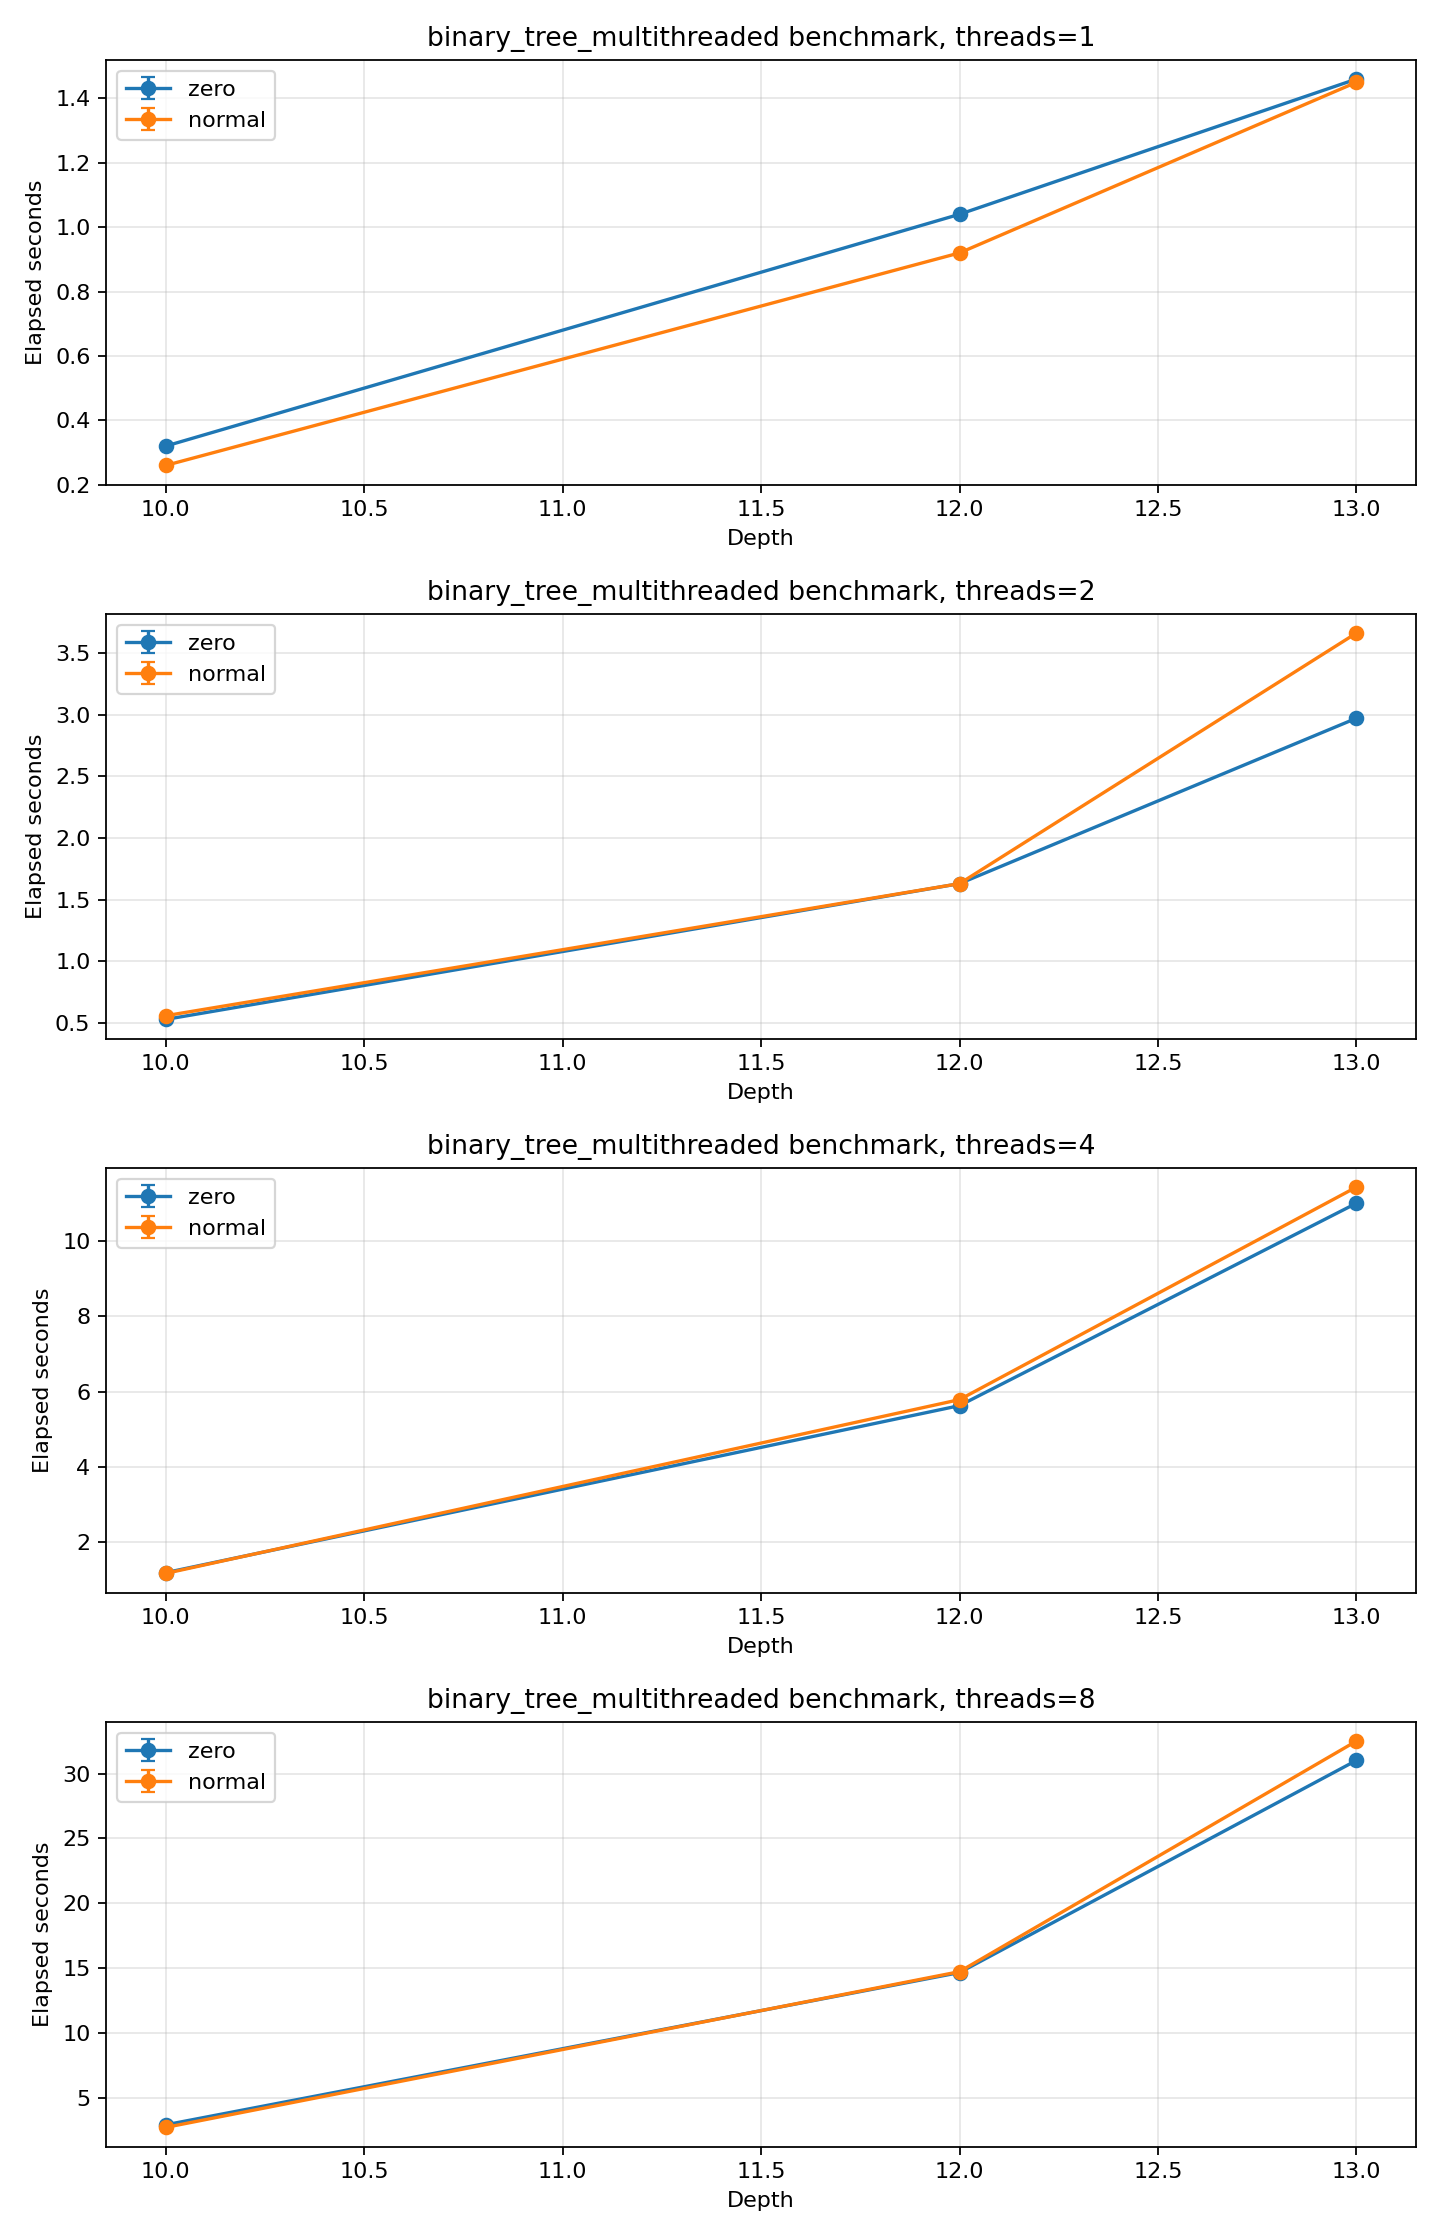
\includegraphics[width=0.75\linewidth]{pilot_normal_vs_zero.png}
  \caption{Pilot benchmark comparing the normal OCaml collector and the
  zero-allocation OxCaml collector.}
  \label{fig:pilot}
\end{figure}

\begin{table}[h]
\centering
\caption{Pilot benchmark summary. Ratio is normal/zero, so values above 1.0
favor the zero-allocation collector.}
\label{tab:pilot}
\begin{tabular}{rrrrr}
\toprule
Depth & Threads & Normal & Zero & Ratio \\
\midrule
10 & 1 & 0.26 & 0.32 & 0.812 \\
10 & 2 & 0.56 & 0.53 & 1.057 \\
10 & 4 & 1.17 & 1.19 & 0.983 \\
10 & 8 & 2.72 & 2.92 & 0.932 \\
12 & 4 & 5.79 & 5.63 & 1.028 \\
13 & 2 & 3.66 & 2.97 & 1.232 \\
13 & 8 & 32.51 & 31.02 & 1.048 \\
\bottomrule
\end{tabular}
\end{table}

The pilot mean over its 12 configurations was 6.403 seconds for
\texttt{normal} and 6.198 seconds for \texttt{zero}. The result suggested that
zero-allocation annotations could help, especially at larger configurations,
but not uniformly.

\subsection{Main Benchmark Results}

\begin{table}[h]
\centering
\caption{Aggregate timing over 32 configurations per variant. Mean is the
arithmetic mean of per-configuration elapsed time.}
\label{tab:aggregate}
\begin{tabular}{lrrrr}
\toprule
Variant & Mean (s) & Min (s) & Max (s) & Faster than normal \\
\midrule
\texttt{normal} & 5.127 & 0.25 & 28.69 & baseline \\
\texttt{zero} & 5.038 & 0.26 & 26.79 & 16 / 32 \\
\texttt{zero\_offheap} & 4.914 & 0.21 & 26.68 & 21 / 32 \\
\texttt{zero\_offheap\_threaded} & 4.919 & 0.23 & 26.11 & 17 / 32 \\
\texttt{zero\_stack\_threaded} & 5.013 & 0.24 & 30.42 & 20 / 32 \\
\bottomrule
\end{tabular}
\end{table}

The best aggregate mean is from \texttt{zero\_offheap}. The threaded off-heap
variant is very close, and the stack-threaded variant is also slightly faster
than the normal baseline on aggregate mean. The largest aggregate gap is only
about 4.2 percent of the normal mean, so it should not be overstated.

\begin{figure}[h]
  \centering
  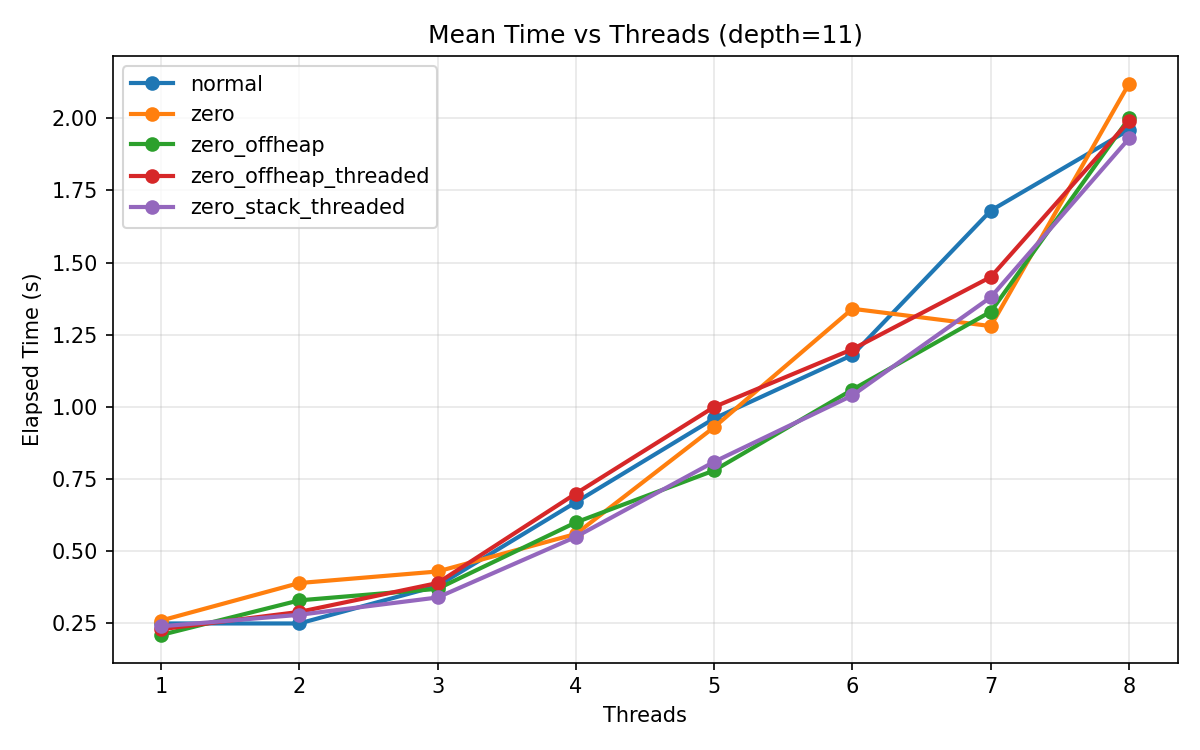
\includegraphics[width=0.48\linewidth]{time_vs_threads_depth_11.png}
  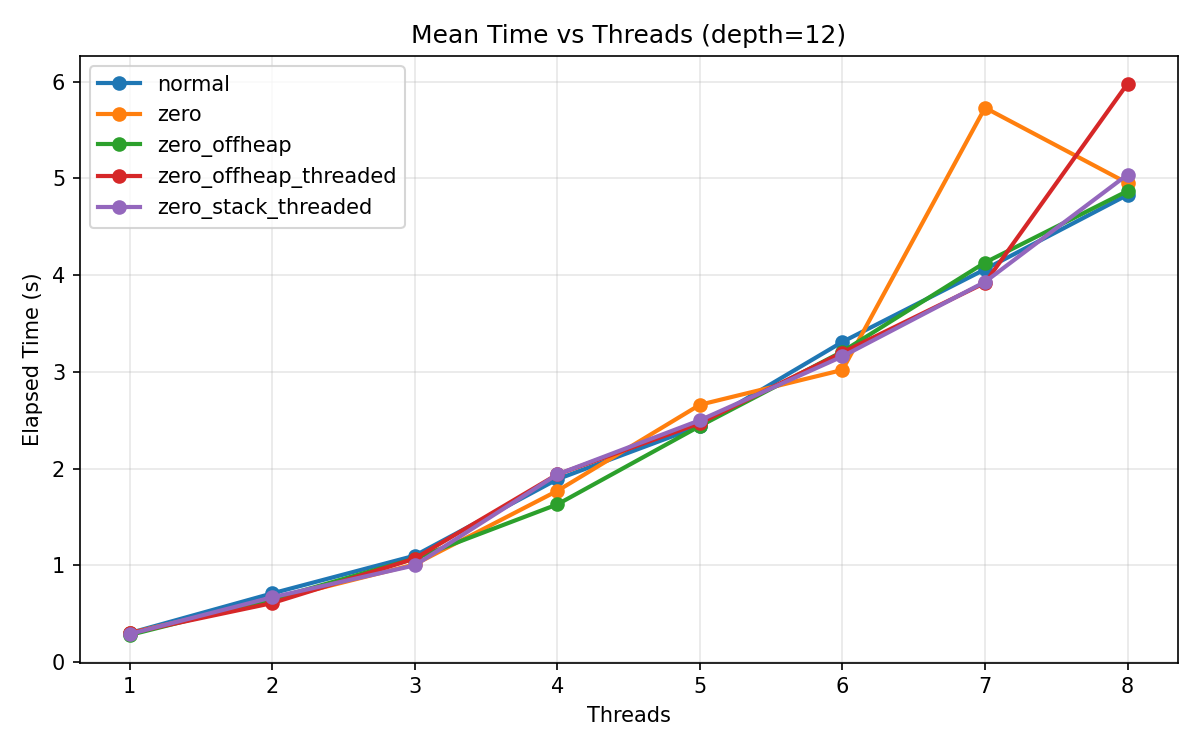
\includegraphics[width=0.48\linewidth]{time_vs_threads_depth_12.png}
  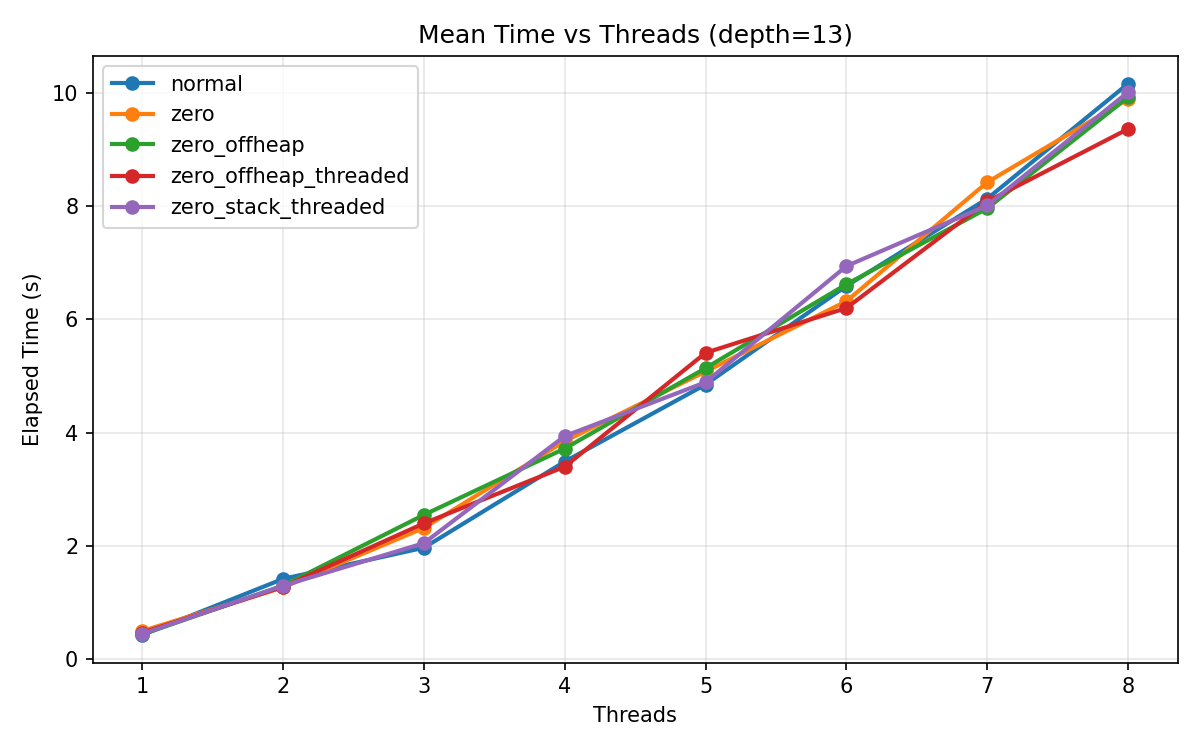
\includegraphics[width=0.48\linewidth]{time_vs_threads_depth_13.png}
  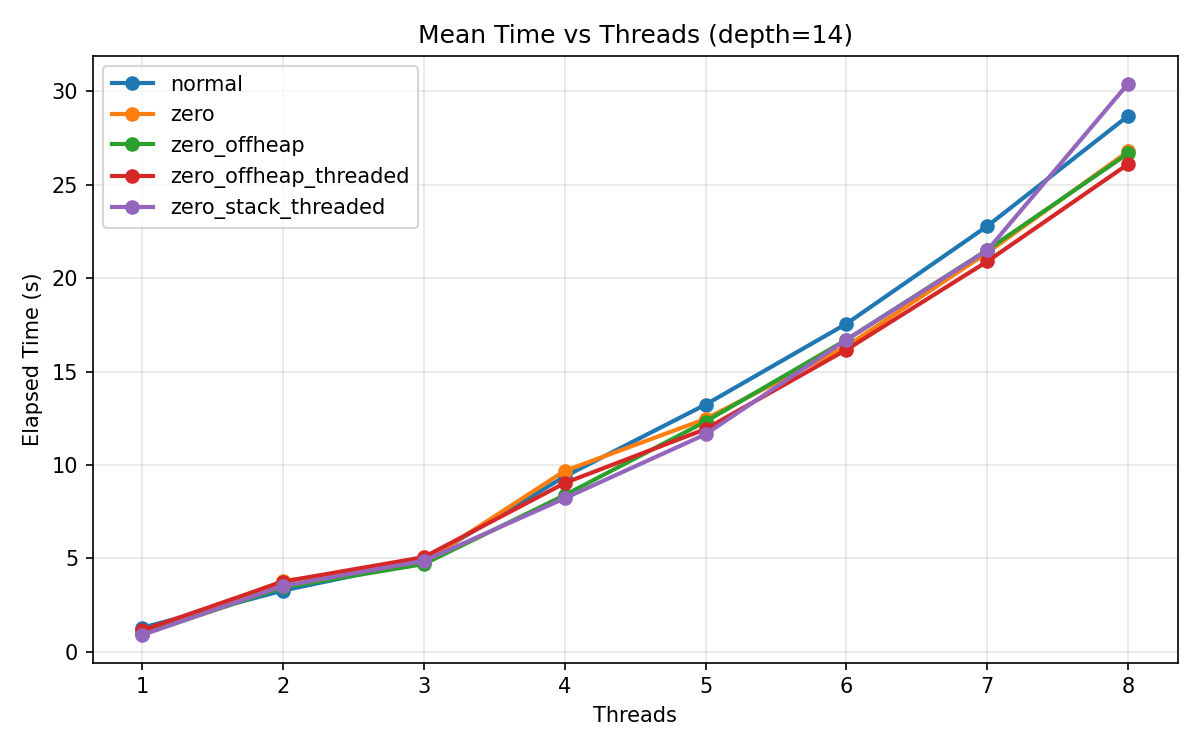
\includegraphics[width=0.48\linewidth]{time_vs_threads_depth_14.png}
  \caption{Elapsed time versus mutator threads for depths 11--14.}
  \label{fig:time-curves}
\end{figure}

\begin{figure}[h]
  \centering
  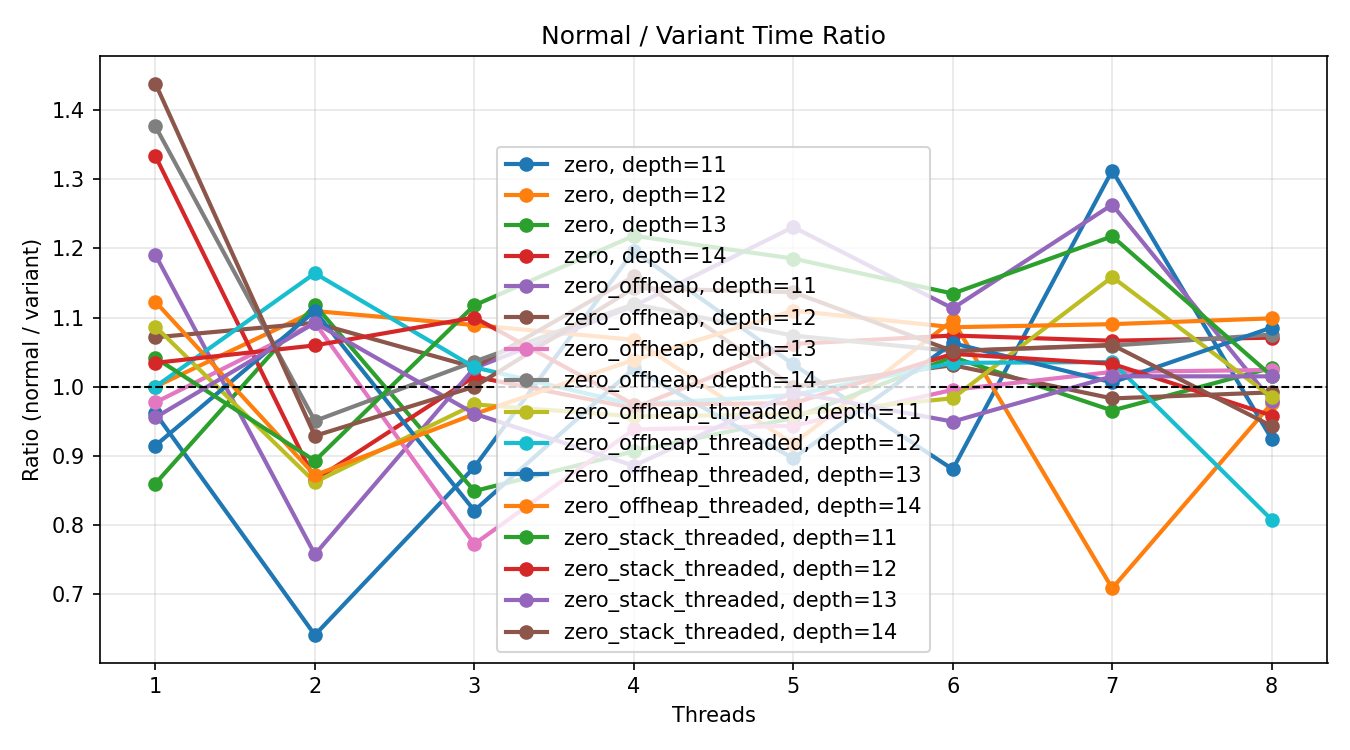
\includegraphics[width=0.88\linewidth]{normal_relative_speedup.png}
  \caption{Normal/variant time ratios. Values above 1.0 mean the variant is
  faster than the normal OCaml baseline.}
  \label{fig:speedup}
\end{figure}

\subsection{Discussion}

The plain \texttt{zero} variant is faster in exactly half of the measured
configurations. This means that zero-allocation annotations alone are not a
universal win. Total elapsed time includes root scanning, C stub calls, object
copying bandwidth, thread coordination, and benchmark scheduling.

The most promising variant is \texttt{zero\_offheap}. It is faster than normal
in 21 of 32 configurations and has the lowest aggregate mean. This supports the
hypothesis that persistent collector metadata should not necessarily live in the
embedded OCaml heap.

Threaded collection is mixed. \texttt{zero\_offheap\_threaded} is strong in some
larger configurations, but the service-thread designs add synchronization, and
that synchronization can outweigh the benefit of a persistent execution context.

\begin{longtable}{rrrrrrr}
\caption{Main benchmark elapsed time by configuration. Times are seconds.}
\label{tab:detail}\\
\toprule
Depth & Threads & Normal & Zero & Offheap & Offheap-thr & Stack-thr \\
\midrule
\endfirsthead
\toprule
Depth & Threads & Normal & Zero & Offheap & Offheap-thr & Stack-thr \\
\midrule
\endhead
11 & 1 & 0.25 & 0.26 & 0.21 & 0.23 & 0.24 \\
11 & 2 & 0.25 & 0.39 & 0.33 & 0.29 & 0.28 \\
11 & 3 & 0.38 & 0.43 & 0.37 & 0.39 & 0.34 \\
11 & 4 & 0.67 & 0.56 & 0.60 & 0.70 & 0.55 \\
11 & 5 & 0.96 & 0.93 & 0.78 & 1.00 & 0.81 \\
11 & 6 & 1.18 & 1.34 & 1.06 & 1.20 & 1.04 \\
11 & 7 & 1.68 & 1.28 & 1.33 & 1.45 & 1.38 \\
11 & 8 & 1.96 & 2.12 & 2.00 & 1.99 & 1.93 \\
12 & 1 & 0.30 & 0.30 & 0.28 & 0.30 & 0.29 \\
12 & 2 & 0.71 & 0.64 & 0.65 & 0.61 & 0.67 \\
12 & 3 & 1.10 & 1.01 & 1.07 & 1.07 & 1.00 \\
12 & 4 & 1.89 & 1.77 & 1.63 & 1.94 & 1.94 \\
12 & 5 & 2.44 & 2.66 & 2.44 & 2.47 & 2.50 \\
12 & 6 & 3.31 & 3.02 & 3.21 & 3.20 & 3.16 \\
12 & 7 & 4.06 & 5.73 & 4.13 & 3.92 & 3.93 \\
12 & 8 & 4.83 & 4.95 & 4.87 & 5.98 & 5.04 \\
13 & 1 & 0.43 & 0.50 & 0.44 & 0.47 & 0.45 \\
13 & 2 & 1.42 & 1.27 & 1.30 & 1.28 & 1.30 \\
13 & 3 & 1.97 & 2.32 & 2.55 & 2.40 & 2.05 \\
13 & 4 & 3.49 & 3.85 & 3.72 & 3.40 & 3.94 \\
13 & 5 & 4.85 & 5.08 & 5.14 & 5.41 & 4.89 \\
13 & 6 & 6.59 & 6.32 & 6.62 & 6.20 & 6.94 \\
13 & 7 & 8.13 & 8.42 & 7.96 & 8.08 & 8.01 \\
13 & 8 & 10.16 & 9.89 & 9.92 & 9.36 & 10.01 \\
14 & 1 & 1.28 & 0.96 & 0.93 & 1.14 & 0.89 \\
14 & 2 & 3.27 & 3.78 & 3.44 & 3.75 & 3.52 \\
14 & 3 & 4.86 & 4.79 & 4.69 & 5.06 & 4.86 \\
14 & 4 & 9.38 & 9.68 & 8.38 & 9.03 & 8.21 \\
14 & 5 & 13.23 & 12.46 & 12.32 & 11.92 & 11.64 \\
14 & 6 & 17.56 & 16.35 & 16.70 & 16.17 & 16.70 \\
14 & 7 & 22.79 & 21.37 & 21.51 & 20.90 & 21.49 \\
14 & 8 & 28.69 & 26.79 & 26.68 & 26.11 & 30.42 \\
\bottomrule
\end{longtable}

% =============================================================================
\section{Reflection on the Use of LLMs}
\label{sec:llm}
% =============================================================================

\paragraph{Tools and models used.}
I used ChatGPT/Codex during the project for code navigation, implementation
planning, debugging, benchmark-script cleanup, plotting-script review, and
report drafting. The LLM was also used to reorganize the repository into a more
standalone shape and to convert benchmark results into tables and prose.

\paragraph{What worked well.}
The most useful assistance was mechanical but time-saving: comparing collector
variants, summarizing benchmark CSVs, identifying which files were build
artifacts, and generating LaTeX tables from result files. The LLM also helped
explain how the zero-allocation and off-heap variants differed in terms of
metadata ownership and runtime coordination.

\paragraph{What did not work.}
The LLM was not reliable as a source of final truth for low-level runtime
behavior. Some early descriptions over-emphasized reference implementations and
made the report sound less independent than the actual project. This was caught
by reviewing the generated report and checking whether the narrative matched
the repository layout.

\paragraph{What was surprising.}
It was useful for quickly turning raw benchmark data into an interpretable
story, but small wording choices mattered a lot. A report can become misleading
if it describes the project as dependent on outside code rather than as a
standalone implementation with its own runtime, benchmarks, and results.

\paragraph{What was difficult.}
The LLM could not replace understanding of the collector invariants. Decisions
about root updates, forwarding, stop-the-world coordination, and whether
zero-allocation annotations were actually meaningful had to be checked against
the code and benchmark behavior.

\paragraph{Your overall assessment.}
The LLM was helpful for acceleration, documentation, and sanity checks, but the
runtime design and performance interpretation still required manual validation.
I would use it again, but only with code review and benchmark verification.

% =============================================================================
\section{Conclusions}
\label{sec:conclusions}
% =============================================================================

The research question was whether an allocation-conscious OCaml/OxCaml
semi-space collector can be competitive with a normal OCaml collector behind a
shared C allocation fast path. The answer from the current evidence is yes, but
with qualifications. The \texttt{zero\_offheap} variant has the best aggregate
mean and beats the normal baseline in most configurations, but the improvement
is small and the benchmark data are single-run.

The main limitation is measurement confidence. The next step is to rerun the
full matrix with 5--10 repetitions per configuration and to separately record
collection count, copied bytes, and GC pause time. That would make it possible
to distinguish collector improvement from mutator scheduling noise and general
runtime overhead.

% =============================================================================
\section*{Contributions}
\label{sec:contributions}
% =============================================================================

\begin{center}
\begin{tabular}{@{}lcl@{}}
\toprule
\textbf{Member} & \textbf{Contribution (\%)} & \textbf{Main responsibilities} \\
\midrule
Aditya Sawant & 100\% & Runtime integration, collector variants, benchmarking, plots, report \\
\midrule
\textbf{Total} & \textbf{100\%} & \\
\bottomrule
\end{tabular}
\end{center}

% =============================================================================
\bibliographystyle{plainurl}
\bibliography{references}
% =============================================================================

\end{document}
